\clearpage

\def\chaptertitle{Introduction}

\lhead{\emph{\chaptertitle}}

\chapter{\chaptertitle}
\label{ch:introduction}

Wybe (pronounced \ipa{["wi.b\textschwa]}, \textsc{WEE-buh}) is a programming language created at the University of Melbourne by \supname~\cite{schachte2015wybe}. Wybe draws inspiration from both logic programming and imperative programming paradigms, taking concepts such as modes and determinism from logic programming into a language with a programming style of imperative languages.

\section{Problem Statement}
\label{sec:problem-statement}

Currently, the Wybe language supports only first-order programming, where all terms have first-order types. In this thesis, we introduce an extension to the Wybe language that supports higher-order programming.

While many languages support higher-order programming, the Wybe language supports features that, to our knowledge, have not been investigated in a higher-order context. One such novel language feature Wybe has is a resource system. Resources in Wybe are akin to global variables in imperative languages or class variables in object-oriented languages. Resources, however, are more constrained in their usage, with each procedure that manipulates a resource requiring being marked as such. 

The resource system has not been investigated in the context of higher-order programming, providing a space in which we can investigate this language feature in a higher-order context. The desired semantics motivate an extension to the intermediate representation that introduces global variables. We aim to extend the Wybe language with our desired semantics of resources and provide novel optimisations enabled by these semantics. 

With these extensions to the Wybe language, we evaluate the performance of the language in terms of execution time and program size, with the existing language as a baseline. While a slow-down may seem detrimental to the utility of a language, higher-order programming increases the expressiveness of a language. The increased expressiveness allows more general programs to be written with less source code and programming effort. Ideally, these overheads should be relatively small in comparison to the overall runtime of a program, lowering the cost of these extensions.

Hence, we aim to answer these research questions:
\begin{enumerate}
  \item How can the Wybe language be extended with higher-order programming?
  \item How can the resource system of Wybe be extended to support higher-order programming while maintaining the guarantees of resources and the expressiveness of higher-order programming?
  \item Do these extensions perform similarly in terms of execution runtime and program size when compared with the existing Wybe language?
\end{enumerate}

\section{Document Outline}
\label{sec:doc-outline}

The remainder of this chapter continues with an overview of the Wybe language. Following, in \cref{ch:lit-review}, we review literature regarding the design an implementation of higher-order programming, type systems, and intermediate representations.

As the Wybe language currently does not support higher-order programming, we introduce new syntactic structures to support higher-order terms in \cref{ch:semantics}. We add functionality to handle common features present with higher-order types, such as partial applications and closures. We define the syntax and semantics of these features, along with the semantics we define for resources in a higher-order context.

In support of a formal basis for the Wybe type system, in \cref{ch:types}, we define a formalised form of the Wybe type system, with declarative semantics. This formalised system provides the basis for which the Wybe type checking algorithm is born. We also outline the heuristics in place for the compiler's type checking algorithm and discuss the higher-order extensions to this algorithm.

In \cref{ch:resources}, we devise an implementation strategy that promotes resources into global variables, motivated by the semantics of resources in a higher-order context. We discuss the existing translation of resources into formal parameters, and also discuss a limitation of globalised resources.

Following, in \cref{ch:lpvm-conversion}, we outline the translation process of the Wybe AST into LPVM, the intermediate representation used within the Wybe compiler, and extend this translation to transform higher-order terms into closures. We also extend LPVM, accordingly to support global variables, and introduce \textit{global flows}, a declarative interface that defines the flow of information of global variables.

In \cref{ch:lpvm-optimisations}, following the extension of LPVM, we extend optimisations currently used within the Wybe compiler to support the extensions with higher-order programming and global variables. We also introduce a novel optimisation that constrains the manipulation of global variables with the aid of global flows.

In \cref{ch:llvm-conversions}, we discuss the translation of the extensions of LPVM into LLVM, the final intermediate representation used by the Wybe compiler. 

Finally, in \cref{ch:experiments}, we investigate the effects of the extended language on various program metrics. This includes the usage of higher-order programming and the implementation of resources using global variables, and the effects on the runtime of programs. We compare the runtime across several programs to gain insight into the performance of the language in the presence of higher-order programming and global variables. We also investigate the size of Wybe programs regarding the usage of higher-order programming and the use of global variables.

\section{The Wybe Language}
\label{sec:wybe-lang}

This section is intended to give the reader an overview of the Wybe language. This should not be considered complete documentation for the language or a complete introduction. It should, however, give the reader an understanding of the syntax and semantics of the Wybe language, to understand the Wybe code fragments that appear throughout the body of this thesis.

The Wybe language's defining principle is a concept called \textit{interface integrity}. Interface integrity is the property that, through the interface of a procedure, all information that flows into and out of a procedure should be known. This ensures that there are no hidden effects of a call --- you can always tell what effects a call could have without needing to look at its implementation. Such effects can be seen from various procedure modifiers also, such as that of purity, and through the explicit usage of resources. 

Wybe employs \textit{copy on write} semantics. Copy on write semantics allows for efficient copying of data by simply copying a reference to the data, while modifications may be slower. In general, data is not copied until it is rewritten, in which case the original data is copied and then is destructively overwritten. As such is possible in Wybe for multiple variables to alias the same data, and to save time copying data, we delay copying data until it is necessary by instead sharing references to the same data when aliased. Only data that is definitely un-aliased can be destructively modified, otherwise, the data must first be copied before the new copy can be destructively modified.

\subsection{Modules}

A Wybe program is divided into discrete sets of items called modules. A module loosely corresponds to a source code file. The file system's structure dictates the module structure between various source files.

Each module contains a series of items, with each having an optional publicity modifier (\texttt{pub}) to indicate this item is visible outside this module. All items are implicitly visible to all submodules. These items are broadly divided into the following categories:

\begin{itemize}
  \item Imports
  \item Top-level code
  \item Submodule declarations
  \item Type constructors or type representation
  \item Procedure and function declarations
  \item Resource declarations
\end{itemize}

\subsubsection*{Imports}

Import statements allow for external modules to be loaded. An import statement (\texttt{use}) is followed by a list of modules, each of which has its public items available for use in the current module. Imports can also be used to load libraries or modules from a foreign language, such as C, allowing the use of foreign code from some other language.

\subsubsection*{Top-level Code}

Top-level code consists of all code that is present at the top-level of a Wybe module. This code is used in the creation of the executable file when compiled, combined with top-level code from other modules. For example, the ``Hello, World!'' program can be written as in \cref{lst:hello-world}, as the \texttt{println} statement exists at the top-level of the program.

\begin{lstlisting}[
  caption={``Hello, World!'' in Wybe.},
  label={lst:hello-world}
]
!println("Hello, world!")
\end{lstlisting}

\subsubsection*{Submodule declarations}

Modules can also contain other modules, called submodules. These submodules implicitly have access to the parent module's items, however, the parent module only has access to the submodule's public items.

\subsubsection*{Type constructors or representation declarations}

Each Wybe module can also be declared as a type. Submodules that are declared as being a \texttt{type} also allow for such constructor declarations. These constructors are further discussed in \cref{ssec:intro-types}.

A Wybe module that is a type can either be an algebraic data type or have a low-level type representation. Low-level type representations allow for primitive types, such as signed or unsigned integers, floating-point numbers, and raw memory addresses to be used within the Wybe language.

\subsubsection*{Procedure and function declarations}

In Wybe, there are two syntactically distinct constructs used to define blocks of code. These are procedures and functions. Procedures allow for the definition of a named block of code, the body, with appropriate inputs and outputs (preceded by a \texttt{?}). Functions are similar, yet have an implicit output value that is the expression that is the body of the function.

\begin{lstlisting}[
  caption={Procedure and function declarations.},
  label={lst:proc-func-decl},
  float=ht
]
def proc(i:int, j:int, ?k:int) {
    ?k = i + j
}

def func(i:int, j:int):int = i + j
\end{lstlisting}

In \cref{lst:proc-func-decl}, we define a procedure, \texttt{proc}, with an equivalent function definition, \texttt{func}. All function definitions are syntactic sugar for procedure definitions in Wybe, and as such, we will focus on procedures throughout the remainder of this thesis.

\subsubsection*{Resource declarations}

Resource declarations allow for a resource to be defined with a given type, with an optional initialisation value. A resource is the replacement of global variables in Wybe and is further detailed in \cref{ssec:intro-resources}.

\subsection{Modes}

Wybe features a strong mode system. The mode system defines which arguments or parameters are treated as inputs, outputs, or both. Each procedure or function declaration defines an interface consisting of a series of parameters, with each parameter prefixed by a flow specifier, which defines the direction data flows via this parameter. A parameter adorned by a preceding \texttt{?} denotes that this parameter is an output to the procedure. For parameters with no prefix, the parameter is considered an input.

A parameter preceded by a \texttt{!} is considered both an input and output. The parameter begins with a value, and can then be modified throughout the body of the procedure, with the final value being passed as an output from the procedure.

In general, a procedure may be defined with any argument in any mode. This means that the number of outputs of a procedure is also unrestricted, unlike in most conventional programming languages.

Multiple procedures can be mode overloaded versions of the same procedure. This allows a Wybe program to define procedures ``in reverse'', similar to how languages such as Prolog and Mercury offer multiple modes. However, Wybe requires \textit{different} procedure bodies for each mode, unlike in Mercury and Prolog where each procedure may be used in different modes but with the same definition by default.

\begin{lstlisting}[
  caption={Procedure declarations with different arities and modes.},
  label={lst:proc-modes},
  float=ht
]
def add( x:int,  y:int, ?z:int) { ?z = x + y }
def add( x:int, ?y:int,  z:int) { ?y = z - x }
def add(?x:int,  y:int,  z:int) { ?x = z - y }
def add(!x:int,  y:int)         { ?x = x + y }

add( 1, ?x, 2) # x = 1  <@\label{lst:proc-modes--1}@>
add(?x,  3, 2) # x = -1 <@\label{lst:proc-modes--2}@>

add(!x, 3) # x = 2 <@\label{lst:proc-modes--3}@>
\end{lstlisting}

In \cref{lst:proc-modes} we define the procedure \texttt{add} with two different arities and 4 different modes. The first is used where the first and second parameters are inputs and the final is an output parameter; the second is used where the second parameter is the output; the third where the first parameter is an output. On line~\ref{lst:proc-modes--1} we use the second defined mode of \texttt{add}, and on line~\ref{lst:proc-modes--2} we use the third defined mode of \texttt{add}. 

The final declaration differs in arity, and has the first argument as an input and an output, and the second as an input. The final call to \texttt{add} on line~\ref{lst:proc-modes--3} uses the previously assigned value of \texttt{x}, and re-assigns \texttt{x} to \texttt{x + 3}.

\subsection{Control Flow}

In Wybe, there are three basic forms of control flow: procedure or function calls, branching, and loops.

Procedure and function calls are the simplest control flow mechanism. A procedure or function can be called by providing the (possibly module qualified) procedure name, followed by a list of arguments with their modes adorned. There may be multiple procedures that match the name (or module) of the call, and which procedure is intended to be called is attempted to be resolved during the type checking process. A procedure or function call binds variables that are outputs of the procedure, with outputs marked with a preceding \texttt{?} as in procedure declarations. Similarly, arguments marked by a preceding \texttt{!} are an input and an output, being reassigned accordingly.

Branching is a simple control flow mechanism that allows computation to branch based on some conditional statement. In general, there may be numerous branches, each with a condition, however, within this thesis, we allow for a branching statement to have two branches, with the second branch being executed if the condition fails to hold. An example conditional branch can be seen in \cref{lst:intro-conditional}.

\begin{lstlisting}[
  caption={Example conditional branches in Wybe.},
  label={lst:intro-conditional},
  float=ht
]
?x = 3
if { x % 2 = 0 ::
    !println("x was even")
| else ::
    !println("x was odd")
}
\end{lstlisting}

Branches bind variables that are bound in all (non-terminal) branches. \textit{I.e.}, if a variable is bound in the condition or the first branch, and it is bound in the second branch, then the variable is bound after the branch.

Loops are the final control structure that we introduce, as seen in \cref{lst:intro-loop}. A \texttt{do} block represents such a loop, a list of instructions that are executed repeatedly. There are two special instructions, \texttt{next} and \texttt{break}, that, respectively, allow for control over the loop structure. The \texttt{next} instruction causes the loop to execute again from the start. The \texttt{break} instruction causes the loop to exit, resuming execution from after the loop body.

\begin{lstlisting}[
  caption={%TC:ignore
    [Example loop in Wybe, printing the ``Bottles of Beer'' song.]%TC:endignore
    Example loop in Wybe, printing the ``Bottles of Beer'' song.~\cite{knuth1984complexity}},
  label={lst:intro-loop},
  float=ht
]
?bottles = 99
do {
    if { bottles = 1 :: 
        !println("1 bottle of beer on the wall, 1 bottle of beer.")
        !print("Take one down and pass it around, ")
        !println("no bottles of beer on the wall")
        break
    | else :: 
        !print(bottles)
        !print(" bottles of beer on the wall, ")
        !print(bottles)
        !println(" bottles of beer.")
        !print("Take one down and pass it around, ")
        ?bottles = bottles - 1 
        !print(bottles)
        !println(" bottles of beer on the wall.")
    }
}
\end{lstlisting}

As a loop is never guaranteed to execute all instructions, a loop will only bind variables that are bound at the end of the loop's body and upon each unconditional \texttt{break}.

\subsection{Types}
\label{ssec:intro-types}

In Wybe, all types are modules, but not all modules are types. Types that are modules have two forms: algebraic data types and low-level representations. The Wybe compiler automatically generates procedures that construct and deconstruct algebraic types into low-level representations which are used in the final stages of code generation in LLVM.

A Wybe module that is an algebraic data type is marked by a \texttt{constructor} declaration, followed by a series of \texttt{|}-separated constructors. Each constructor consists of a name and a (possibly empty) list of fields, each of which has a type and an optional name. Constructors are much like that in a language such as Haskell, lacking any source-defined body, contrasting constructors in a language such as Java where the constructor is defined in the source code. Named fields implicitly define a getter and setter procedure, which are used to get the value of the field and to construct a new value with the same values up to the field that is set, respectively. 

For example, in \cref{lst:intro-adt}, the \texttt{number} type implicitly defines constructors and deconstructors for the \texttt{natural} and \texttt{rational} constructors, and a (\texttt{test}) procedure to get the \texttt{nat} or \texttt{rat} field from a respective value of type \texttt{number}, with these procedures failing if the wrong constructor was used.

\begin{lstlisting}[
  caption={Example abstract data types in Wybe.},
  label={lst:intro-adt},
  float=ht
]
type number { natural(nat:int) | rational(rat:float) }
type tree(X) { nil | node(left:tree(X), X, right:tree(X)) }
\end{lstlisting}

Wybe also supports generic programming. Type variables are declared in the source code as a single uppercase letter followed by zero or more digits (\texttt{[A-Z][0-9]*}) (\textit{e.g.}, \texttt{X} in \cref{lst:intro-adt}). Algebraic types can also be defined polymorphically, being defined with some number of type parameters, which can then be instantiated to some other type when the type is used. An example of such a polymorphic type is the \texttt{tree} type in \cref{lst:intro-adt}, which is defined recursively.

As Wybe uses a static type system, the types of all variables are checked for correctness at compile time. This ensures that a type error cannot occur at runtime. Wybe also features type inference. This allows for the types of variables in a program to be inferred, permitting correctly typed programs to be compiled while lacking type annotations.

One of the distinctive features of the Wybe type system is that of how types can be inferred. The property that is distinct in the Wybe type systems is that types of procedure parameters can only be inferred from the declarations of a procedure itself, not from the contexts where the procedure is called. This property of the Wybe type system makes it distinct from other type systems where the types of a procedure's parameters can be inferred by the contexts wherein it is called. 

\subsection{Resources}
\label{ssec:intro-resources}

Resources are a novel parameter-passing mechanism featured in the Wybe language. Resources are similar to global variables found in imperative languages, class variables found in object-oriented languages, or the state monad seen in functional languages. Unlike global variables, however, usage of a resource is explicit, and as such stronger optimisations can be performed than could with a global variable.

The intent of a resource is to store a value which may be used throughout the computation, being passed through many calls, yet there is only one of these values in a given computation. Whereas conventionally arguments are passed positionally, a resource is a parameter that is passed implicitly by name, which allows the programmer to automatically thread a resource's state through calls. The value of a resource can be accessed as if it were a variable, and (re-)assignments of this variable will (re-)assign the resource.

A procedure can be defined to \texttt{use} some resource. This is annotated in the interface of each procedure, with each used resource having an accompanying flow. To call a procedure that uses some resource, then the resource must be in scope, and the call to the resourceful procedure must be marked with a preceding \texttt{!} to ensure a reader is aware a resource is being used. A resource is in scope if it is called within a procedure that uses the same resource, or in a scoped \texttt{use} block. 

For a resourceful procedure call, some conditions must be met. For inwards flowing resources, the resource is considered an input to the procedure. This means that the resource must not only be in scope for the call to be valid but also must be bound to a value before the call. The value of the resource after the call will be the same as after the call. Outwards flowing (\texttt{?}) resources allow for the procedure to be called where the resource is in scope but not necessarily bound. The resource is then bound after the call. Finally, a resource with an input and output flow (\texttt{!}) must not only be in scope but also must be bound before the call. The value of the resource may change after the call. Examples of each flow and correct usage can be found in \cref{lst:ss--resource-flow}. 

\begin{lstlisting}[
  caption={Example resource flows},
  label={lst:ss--resource-flow},
  float=ht
]
resource res:int

def in(?x:int) use res {  # value of res can be used 
    ?x = res             
    ?res = res + 1
}
def out(x:int) use ?res { # value of res can only be used once set 
    x = ?res
}
def inout use !res {      # value of res can be used, and modified
    ?res = res = 1
}

use res in {
    ?res = 1  # assign res a value
    !in(?x)   # res is implicitly passed in, also remains unchanged
    !out(x)   # res is implicitly passed out, value before is irrelevant
    !inout(x) # res is implicitly passed in/out
}
\end{lstlisting}

Resource usage can also be scoped in a \texttt{use} block. All resources that are named for the \texttt{use} block are in scope for the entirety of the intervening statements. Scoped resources are considered bound if a variable of the same name was bound just before the \texttt{use} block, otherwise, if there was no variable bound before the block, the resource is considered unbound. The value of any resource (or variable of the same name) after the block is saved before the block and restored after. If the resource was unbound before the scope, the resource remains unbound after the scope. In \cref{lst:intro-resources} the \texttt{strings} resource is used in a \texttt{use} block, introducing a scope wherein the resource can be used.

In the standard library of the Wybe language, a resource \texttt{io} is defined. The \texttt{io} resource is designed to provide a pure interface via which declarative I/O is performed, with the resource representing the state of the entire world. Each I/O procedure is defined with \texttt{use !io} in their interface, which ensures that the state is fed through the entire computation where I/O is performed. The \texttt{io} resource has a \textit{phantom} type, being a 0-bit integer type, that is used throughout compilation to ensure the ordering of I/O operations while containing no information, and as such is eliminated in the late stages of code generation. This provides declarative I/O with zero overhead.

\begin{lstlisting}[
  caption={Example resource and \texttt{use} block usage.},
  label={lst:intro-resources},
  float=ht
],
# declare `strings` resource, a list of strings
resource strings:list(string)

type tree(T) { pub nil | node(left:tree(T), value:T, right:tree(T)) }

# prepend a single string to the head of `strings`
def collect(str:string) use !strings {
    ?strings = [str | strings]
}

# add all strings from the tree to the start of `strings`.
# traverse right-to-left to ensure the strings are accumulated in-order
def collect(tree:tree(string)) use !strings {
    if { tree = node(?left, ?str, ?right) :: 
        !collect(right)
        !collect(str)
        !collect(left)
    }
}

# create a scope where we can use `strings`
use strings in {
    # bind `strings` to the empty list
    ?strings = []
    # construct a tree
    ?tree = node(node(nil, "a", nil),       # tree:   "b"
                 "b",                       #        /   \
                 node(nil,                  #      "a"   "c"
                     "c",                   #               \
                     node(nil, "d", nil)))) #               "d"
    # collect strings from the tree
    !collect(tree)
    # after: strings = ["a", "b", "c", "d"]
}
\end{lstlisting}

In \cref{lst:intro-resources} we see an example of resource usage. The resource, \texttt{strings}, is declared with the type of \texttt{list(string)}. We define two procedures that \texttt{use} the \texttt{strings} resource in the in/out mode. The first procedure, \texttt{collect(str:string)}, prepends a single string to the \texttt{strings} resource. In this procedure, we use the resource by referencing the variable of the same name.

The second procedure, \texttt{collect(tree:tree(string))}, traverses a defined \texttt{tree} type. We begin by deconstructing the \texttt{tree} if it is of the \texttt{node} constructor, into a \texttt{left} tree, the node's value, \texttt{str}, and a \texttt{right} tree. We then recursively \texttt{collect} the strings from the \texttt{right} tree, append the value \texttt{str}, and recursively collect the strings from the \texttt{left} tree. In this procedure we do not refer to the resource by name, instead the state of the resource is passed implicitly.

In the top-level code, we create a scope where we can \texttt{use} the \texttt{strings} resource. Inside this scope the \texttt{strings} resource can be used, but it is not bound to a value. We bind the \texttt{strings} resource to the empty list \texttt{[]}.

We then \texttt{collect} all strings from a \texttt{tree} structure. This results in the \texttt{strings} resource having a value of \texttt{["a", "b", "c", "d"]}, which is a left-to-right ordering of the elements of the \texttt{tree}.

\subsection{Determinism}

In Wybe, the determinism of a procedure is a property of a procedure that dictates two properties: the number of solutions of a procedure, and if the procedure can fail. Determinisms allow for the programmer to declare where a procedure may fail to produce a result, with this property being used by the compiler to generate code that handles such failures appropriately.

The determinism system of Wybe is similar to other languages, such as Mercury, however, differs in its current state, lacking the \texttt{nondet} and \texttt{multi} determinisms. In Wybe, there are four determinisms, as outlined in \cref{fig:intro-detism}. The properties of each determinism are checked by the compiler to ensure correctness.

The different determinisms of a procedure call are valid in different determinism contexts. For a context to be considered to have a determinism, it may be that the context is inside a procedure with said determinism, or in the case of a conditional statement's condition, the context has the \texttt{test} context.

\begin{figure}[ht]
  \centering
  \begin{subfigure}[htb]{0.49\textwidth}
    \centering 
    \begin{tabular}{cl|cc}
        & & \multicolumn{2}{c}{Maximum number of solutions} \\
        & & 0 & 1 \\
      \hline
      \multirow{2}{*}{Can fail?}
        & No  & \texttt{terminal} & \texttt{det}  \\
        & Yes & \texttt{failing}  & \texttt{test} \\
    \end{tabular}
    \vfill
    \caption{Properties of determinisms.}
    \label{sfig:detism-table}
  \end{subfigure}\hfill
  \begin{subfigure}[htb]{0.49\textwidth}
    \centering
    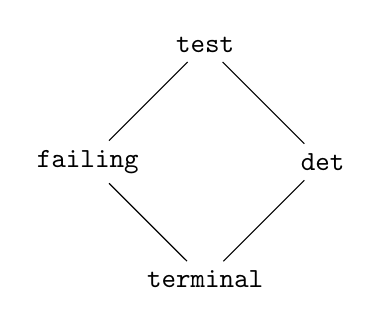
\begin{tikzpicture}[
      node distance = 6em
    ]
      \node (test)                              {\texttt{test}};
      \node (failing)  [below left of=test]     {\texttt{failing}};
      \node (det)      [below right of=test]    {\texttt{det}};
      \node (terminal) [below right of=failing] {\texttt{terminal}};
      \draw (test)    -- (failing);
      \draw (test)    -- (det);
      \draw (det)     -- (terminal);
      \draw (failing) -- (terminal);
    \end{tikzpicture}
    \caption{The determinism lattice.}
    \label{sfig:detism-lattice}
  \end{subfigure}
  \caption{The determinism system of Wybe.}
  \label{fig:intro-detism}
\end{figure}

By default, a procedure has the \texttt{det} determinism. Such a procedure behaves much like procedures in regular languages. That is, the procedure cannot fail and succeeds exactly once. \texttt{det} procedure can be called in any context.

The \texttt{test} (or \texttt{partial}) determinism denotes a procedure that \texttt{may} fail to produce a result. \texttt{test} procedures are valid in both \texttt{test} and \texttt{failing} contexts. An example \texttt{test} call can be found in \cref{lst:ss--test}.

Optionally, a \texttt{test} procedure call can be called with an out-flowing Boolean-typed variable, reifying the \texttt{test} procedure call into a \texttt{det} procedure call. This variable is true if the procedure succeeded, otherwise, it is false. Conversely, if the final parameter of a \texttt{det} procedure call is an output with a Boolean type, and the corresponding argument is omitted, the \texttt{det} procedure call can be de-reified into a \texttt{test} procedure call. 

\begin{lstlisting}[
  caption={Example \texttt{test} procedure, usage and reification.},
  label={lst:ss--test},
  float=ht
]
def {test} even(n:int) { n % 2 = 0 }

# if condition is a test
if { even(3) :: !println("that's odd!") }

# reified test
even(4, ?succeeded)
if { succeeded :: !println("that's even!") }
\end{lstlisting}

The \texttt{failing} determinism denotes a procedure that will always fail, providing zero solutions. A built-in \texttt{failing} procedure is the \texttt{fail} procedure, which takes zero arguments and fails. \texttt{failing} procedures are valid in both \texttt{failing} and \texttt{test} contexts.

The final determinism in Wybe is the \texttt{terminal} determinism. A \texttt{terminal} procedure is a procedure that will never succeed nor fail, providing zero solutions. This means that, when a \texttt{terminal} procedure is called, all subsequent statements will not execute. A \texttt{terminal} procedure can be called in any context. Example \texttt{terminal} procedures include infinite loops and procedures that can exit the program such as the \texttt{error} procedure.

\subsection{Purity}

\textit{Purity} is the property of a procedure or function to perform identically when provided identical inputs and to have no observable side effects. A pure procedure is said to be an analogue of a mathematical function, and knowledge of a procedure's purity is of interest internally to the compiler. As a pure procedure behaves identically on identical inputs, multiple invocations of the same pure procedure are subject to common sub-expression elimination. Common sub-expression elimination allows a previously computed output of some previous invocation of the same procedure with identical inputs to be reused, eliminating the successive call to the pure procedure.

All Wybe procedures are \texttt{pure} by default and can call other \texttt{pure} (and \texttt{semipure} procedures). \texttt{pure} procedures are subject to call re-ordering, call omission, and common sub-expression elimination. All calls to non-pure (\texttt{semipure} or \texttt{impure}) procedures are marked by a preceding \texttt{!}, as shown in \cref{lst:purity-call}. This is to remind the reader that the call is not pure.


\begin{lstlisting}[
  caption={Example non-pure procedure and call.},
  label={lst:purity-call},
  float=ht
]
def {semipure} update_string(s:c_string, i:int, c:char) {
    foreign lpvm {impure} mutate(s, ?s, i, 1, 1, 0, c)
}

# create a C-style string
?str = c_string("abc",,"xyz")
!update_string(str, 1, 'B') 
\end{lstlisting}

Each procedure can have one of three purity modifiers: \texttt{pure}, \texttt{semipure}, and \texttt{impure}. An \texttt{impure} procedure is free to call procedures of all purity levels. A \texttt{semipure} procedure has the property that it is allowed to call all levels of purity, however, is subject to call-reordering, a property that \texttt{impure} procedures do not have. Like regular pure procedures, procedures with an explicit \texttt{pure} modifier can be subject to call re-ordering, call omission, and common sub-expression elimination, however, are allowed to call \texttt{impure} procedures within its body. 

These optimisations are available for pure procedures due to the property that a pure procedure acts as a mathematical function. Pure procedures have no side effects, always producing the same outputs with identical inputs. Call-reordering allows for re-ordered calls to be optimised differently, exploiting redundancies that allow for other optimisations to produce more optimised code. With Wybe's copy-on-write semantics, re-ordering may allow for these semantics to be violated if re-ordering produces equivalent code with un-aliased memory. An example of when this optimisation can and cannot be performed with re-ordered pure code can be found in \cref{lst:purity-order}.

\begin{figure}
  \setcaptiontype{lstlisting}
  \begin{minipage}[t]{.48\textwidth}
    \begin{lstlisting}
reverse(ls, ?rev)
sum(ls, ?ls_sum)
sum(rev, ?rev_sum)
\end{lstlisting}
    \subcaption{\texttt{rev} cannot destructively re-use the allocated memory of \texttt{ls}, as \texttt{ls} is used after.}
    \label{slst:purity-rev-bad}
  \end{minipage}\hfill
  \begin{minipage}[t]{.48\textwidth}
    \begin{lstlisting}[numbers=none]
sum(ls, ?ls_sum)
reverse(ls, ?rev)
sum(rev, ?rev_sum)
\end{lstlisting}
    \subcaption{\texttt{rev} can destructively re-use the allocated memory of \texttt{ls}.}
    \label{slst:purity-rev-good}
  \end{minipage}
  \caption{Example calls that, when re-ordered, can produce more optimal code.}
  \label{lst:purity-order}
\end{figure}

\section{Current Compiler Architecture Overview}
\label{sec:current-compiler-arch}

The Wybe compiler can broadly be decomposed into three major stages. These stages correspond to an intermediate representation of a given program: the AST, LPVM, and LLVM. 

The first stage represents a Wybe program in an AST form, being an abstract representation of the syntax of the Wybe language. This component performs manipulation of the source code, performing tokenisation and parsing, producing a denormalised AST. The denormalised AST is then normalised, introducing implicit procedures for declared types (constructors, deconstructors, getters, setters, \textit{etc.}) and transforming function definitions into equivalent procedure definitions. Normalisation also includes a flattening pass of the AST, reducing complex AST constructs such as \texttt{for} loops into simpler, semantically equivalent, forms.

This stage proceeds with type and mode checking. Type and mode checking in tandem are used to disambiguate overloading, resolving which instance of a procedure the call corresponds to. This stage attempts to infer the type of any terms that are not explicitly types and checks that all types are correct in a given program. Mode checking is responsible for the final overloading resolution after all terms have been typed, and for ensuring that variables and resources are appropriately bound before use. Resources are then transformed into positional parameters and arguments in the following pass.

The next pass of the compiler performs more aggressive flattening called \textit{unbranching}. Here the compiler transforms the AST to a restricted form that only contains procedure calls and tailing conditional branches, transforming loops into recursive procedures. All calls after unbranching are also transformed into equivalent deterministic calls, by reifying calls that are not deterministic with the following branch. After unbranching, the AST resembles LPVM, and as such we perform a pass that transforms the AST into LPVM. 

Following the transformation into LPVM, we enter the second major stage. This stage is concerned with the analysis and transformations of the LPVM intermediate representation of a Wybe program. The primary optimisation pass performed on LPVM performs inlining, building upon the general optimisation framework built into the compiler, the \textit{body builder} which performs amongst other optimisations value propagation, and neededness analysis.

This pass also performs alias analysis, inferring which variables alias the same data. This analysis is used to transform, when possible, calls that have certain un-aliased arguments. Due to Wybe's copy-on-write semantics, a program can perform redundant copies on certain writes where the old copy is unused. These transformations allow for code to be transformed to violate the copy-on-write semantics due to this redundancy, however, retaining the same operational semantics. This analysis is also used to perform compile-time garbage collection if memory is un-aliased and unused, then can be reused by some later memory allocation~\cite{chen2020multiple}.

Finally, we leverage the LLVM compiler~\cite{lattner2004llvm} to perform the final code generation. We also make use of the optimisation passes implemented in the LLVM compiler, further producing more optimal code. This ultimately produces the object files, used for more efficient incremental compilation~\cite{ranjan2016incremental}, and binary executable files.
